\chapter{Diagrammi dei casi d'uso}
\noindent Il rettangolo nel diagramma rappresenta sempre il sistema \textbf{Wiki Collaborativo per Appunti}, ovvero il \textbf{soggetto}. La modellazione dei casi d’uso è stata articolata in base ai ruoli interpretati dagli attori esterni, al fine di evidenziare il \textbf{disaccoppiamento} tra le funzionalità pubbliche e quelle riservate:

\begin{itemize}[]
    \item \textbf{Visitatore}: rappresenta l'utente non autenticato che consulta il materiale.
    \item \textbf{Studente}: utente autenticato con permessi di contribuzione.
    \item \textbf{Amministratore}: ruolo preposto alla gestione strutturale di corsi e argomenti.
\end{itemize}

\noindent Sotto il profilo della modellazione, sia il ruolo \textbf{Studente} che il ruolo \textbf{Amministratore} sono rappresentati come generalizzazioni del \textbf{Visitatore}. Questa astrazione permette di indicare che entrambi i ruoli autenticati ereditano implicitamente tutti i casi d’uso di consultazione e ricerca (\textbf{RF3, RF4, RF9}) senza appesantire graficamente il diagramma con linee ridondanti.
Tuttavia, si evidenziano due importanti eccezioni alla gerarchia dei permessi:


\begin{itemize}[]
    \item \textbf{Esclusione del caso d'uso Registrazione (RF1)}: Una volta autenticati, né lo \textbf{Studente} né l'\textbf{Amministratore} possono accedere alla funzione di registrazione, in quanto lo stato di utente loggato è logicamente incompatibile con la creazione di un nuovo account.
    \item \textbf{Vincoli sulla creazione degli account}: In linea con i requisiti di sicurezza, la funzione di registrazione pubblica è limitata esclusivamente al ruolo \textbf{Studente}. Il ruolo \textbf{Amministratore} non può essere ottenuto tramite registrazione autonoma (per prevenire scalate di privilegi non autorizzate), ma viene gestito esclusivamente a livello di persistenza tramite l'inserimento manuale o script di inizializzazione nel database.
\end{itemize}

\noindent Ho diviso i diagrammi per attore per rendere più chiara la separazione delle responsabilità e dei permessi di accesso, facilitando la tracciabilità tra i requisiti funzionali e le interazioni modellate .

\section{Dettagli del Caso d'Uso UC1}

\begin{figure}[H] % h=here, t=top, b=bottom, p=page [8, 9]
    \centering
    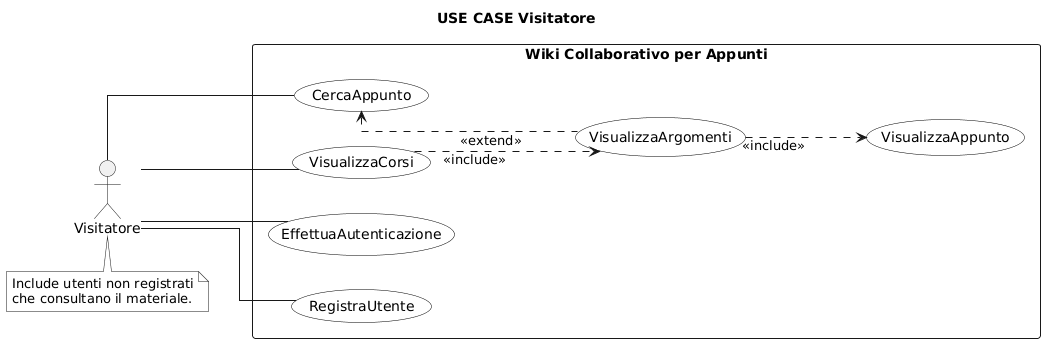
\includegraphics[width=1\textwidth]{UseCase/visitatore.png} % [10, 11]
    \caption{UC1 - Diagramma dei casi d'uso per l'attore Visitatore}
    \label{fig:uc_visitatore} % [12, 13]
\end{figure}

\begin{table}[H]
    \small
    \caption{Specifica del caso d'uso per RF1: RegistraUtente}
    \begin{tabularx}{\textwidth}{@{}l X@{}}
        \toprule
        \textbf{ID} & 1 \\
        \midrule
        \textbf{Nome} & \textbf{RegistraUtente} \\
        \midrule
        \textbf{Descrizione} & Permette a un nuovo utente di creare un account fornendo email e password. \\
        \midrule
        \textbf{Attori} & Visitatore. \\
        \midrule
        \textbf{Precondizioni} & L'utente non è registrato. \\
        \midrule
        \textbf{Flusso Principale} & 
        1. L'utente seleziona la funzione di registrazione. \newline
        2. L'utente inserisce email e password. \newline
        2. Il sistema valida il formato dei dati (es. email valida). \newline
        4. Il sistema esegue l'hashing della password per sicurezza. \newline
        5. Il sistema memorizza i dati nel database. \\
        \midrule
        \textbf{Postcondizioni} & Un nuovo account è stato creato con successo. \\
        \midrule
        \textbf{Flussi Alternativi} & \textbf{A1. Email già presente:} Il sistema informa l'utente che l'email è già registrata e interrompe la procedura. \\
        \bottomrule
    \end{tabularx}
\end{table}

\begin{table}[H]
    \small
    \caption{Specifica del caso d'uso per RF2: EffettuaAutenticazione}
    \begin{tabularx}{\textwidth}{@{}l X@{}}
        \toprule
        \textbf{ID} & 2 \\
        \midrule
        \textbf{Nome} & \textbf{EffettuaAutenticazione} \\
        \midrule
        \textbf{Descrizione} & Consente all'utente di accedere al sistema tramite le proprie credenziali. \\
        \midrule
        \textbf{Attori} & Visitatore. \\
        \midrule
        \textbf{Precondizioni} & L'utente deve possedere un account registrato. \\
        \midrule
        \textbf{Flusso Principale} & 
        1. L'utente accede alla funzione di login. \newline
        2. L'utente inserisce email e password. \newline
        3. Il sistema confronta le credenziali con quelle nel database. \newline
        4. Il sistema avvia una sessione autenticata. \\
        \midrule
        \textbf{Postcondizioni} & L'utente è autenticato e in base al suo ruolo può accedere alle funzioni di creazione/modifica. \\
        \midrule
        \textbf{Flussi Alternativi} & \textbf{A1. Credenziali errate:} Il sistema nega l'accesso e mostra un messaggio di errore. \\
        \bottomrule
    \end{tabularx}
\end{table}

\begin{table}[H]
    \small
    \caption{Specifica del caso d'uso per RF3: VisualizzaCorsi}
    \begin{tabularx}{\textwidth}{@{}l X@{}}
        \toprule
        \textbf{ID} & 3 \\
        \midrule
        \textbf{Nome} & \textbf{VisualizzaCorsi} \\
        \midrule
        \textbf{Descrizione} & Permette di consultare l'elenco completo dei corsi disponibili nel Wiki. \\
        \midrule
        \textbf{Attori} & Visitatore. \\
        \midrule
        \textbf{Precondizioni} & Il sistema è accessibile. \\
        \midrule
        \textbf{Flusso Principale} & 
        1. L'utente accede alla pagina principale. \newline
        2. In automatico il sistema recupera i nomi dei corsi dal database. \newline
        3. Il sistema mostra l'elenco dei corsi all'utente. \\
        \midrule
        \textbf{Postcondizioni} & L'utente visualizza l'elenco dei corsi. \\
        \bottomrule
    \end{tabularx}
\end{table}

\begin{table}[H]
    \small
    \caption{Specifica del caso d'uso per RF4: VisualizzaArgomenti}
    \begin{tabularx}{\textwidth}{@{}l X@{}}
        \toprule
        \textbf{ID} & 4 \\
        \midrule
        \textbf{Nome} & \textbf{VisualizzaArgomenti} \\
        \midrule
        \textbf{Descrizione} & Permette di navigare tra gli argomenti associati a un corso specifico. \\
        \midrule
        \textbf{Attori} & Visitatore. \\
        \midrule
        \textbf{Precondizioni} & L'utente ha selezionato un corso (3). \\
        \midrule
        \textbf{Flusso Principale} & 
        1. L'utente seleziona un corso. \newline
        2. Il sistema recupera gli argomenti legati a quel corso. \newline
        3. Il sistema mostra la lista degli argomenti di quel corso. \\
        \midrule
        \textbf{Postcondizioni} & L'utente visualizza gli appunti collegati a quell'argomento. \\
        \bottomrule
    \end{tabularx}
\end{table}

\begin{table}[H]
    \small
    \caption{Specifica del caso d'uso per RF5: VisualizzaAppunto}
    \begin{tabularx}{\textwidth}{@{}l X@{}}
        \toprule
        \textbf{ID} & 5 \\
        \midrule
        \textbf{Nome} & \textbf{VisualizzaAppunto} \\
        \midrule
        \textbf{Descrizione} & Mostra il contenuto di un appunto in formato HTML renderizzato. \\
        \midrule
        \textbf{Attori} & Visitatore. \\
        \midrule
        \textbf{Precondizioni} & L'utente ha selezionato un corso e un argomento (4). \\
        \midrule
        \textbf{Flusso Principale} & 
        1. L'utente seleziona un appunto. \newline
        2. Il sistema recupera il testo (Markdown/Plain text) dal database. \newline
        3. Il sistema converte il testo in HTML e lo visualizza. \\
        \midrule
        \textbf{Postcondizioni} & L'utente visualizza l'appunto renderizzato. \\
        \bottomrule
    \end{tabularx}
\end{table}

\begin{table}[H]
    \small
    \caption{Specifica del caso d'uso per RF9: CercaAppunto}
    \begin{tabularx}{\textwidth}{@{}l X@{}}
        \toprule
        \textbf{ID} & 9 \\
        \midrule
        \textbf{Nome} & \textbf{CercaAppunto} \\
        \midrule
        \textbf{Descrizione} & Permette la ricerca di appunti tramite titolo, contenuto o corso. \\
        \midrule
        \textbf{Attori} & Visitatore. \\
        \midrule
        \textbf{Precondizioni} & Il sistema è operativo. \\
        \midrule
        \textbf{Flusso Principale} & 
        1. L'utente inserisce una stringa nella funzione di ricerca. \newline
        2. Il sistema interroga il database cercando corrispondenze nei titoli. \newline
        3. Il sistema mostra i risultati filtrati. \\
        \midrule
        \textbf{Postcondizioni} & L'utente seleziona un appunto dai risultati (prosegue con 5). \\
        \bottomrule
    \end{tabularx}
\end{table}


\section{Dettagli del Caso d'Uso UC2}

\begin{figure}[H] % h=here, t=top, b=bottom, p=page [8, 9]
    \centering
    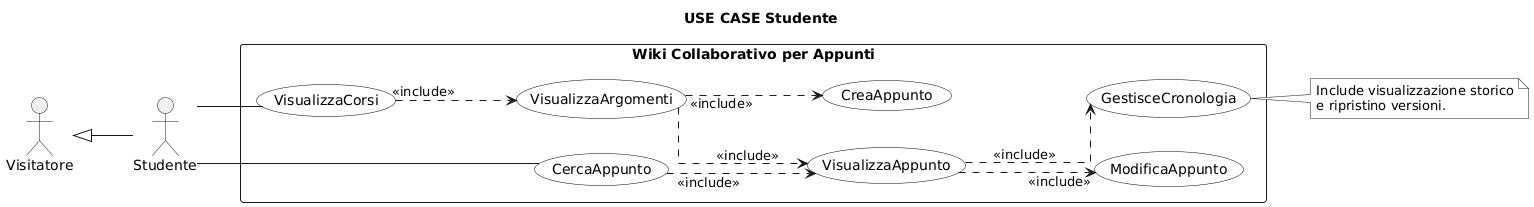
\includegraphics[width=1\textwidth]{UseCase/stud.png} % [10, 11]
    \caption{UC2 - Diagramma dei casi d'uso per l'attore Studente}
    \label{fig:uc_studente} % [12, 13]
\end{figure}

\begin{table}[H]
    \small
    \caption{Specifica del caso d'uso per RF6: CreaAppunto}
    \label{tab:spec_uc6}
    \begin{tabularx}{\textwidth}{@{}l X@{}}
        \toprule
        \textbf{ID} & 6 \\
        \midrule
        \textbf{Nome} & \textbf{CreaAppunto} \\
        \midrule
        \textbf{Descrizione} & Permette a un utente autenticato di inserire un nuovo appunto nel sistema associandolo a un corso e a un argomento specifico. \\
        \midrule
        \textbf{Attori} & Studente. \\
        \midrule
        \textbf{Precondizioni} & L'utente ha effettuato il login (2) e si trova nella sezione di visualizzazione degli appunti per argomento (4). \\
        \midrule
        \textbf{Flusso Principale} & 
        1. L'utente seleziona la funzione "Crea Nuovo Appunto". \newline
        2. L'utente inserisce il titolo dell'appunto. \newline
        3. L'utente inserisce il contenuto testuale (Markdown o Plain Text). \newline
        4. L'utente conferma il salvataggio. \newline
        5. Il sistema valida i dati, memorizza l'appunto e associa l'ID dell'autore. \\
        \midrule
        \textbf{Postcondizioni} & Il nuovo appunto è persistente nel database. \\
        \midrule
        \textbf{Flussi Alternativi} & \textbf{A1. Dati mancanti:} Se il titolo è vuoto, il sistema non procede al salvataggio. \\
        \bottomrule
    \end{tabularx}
\end{table}

\begin{table}[H]
    \small
    \caption{Specifica del caso d'uso per RF7: ModificaAppunto}
    \label{tab:spec_uc7}
    \begin{tabularx}{\textwidth}{@{}l X@{}}
        \toprule
        \textbf{ID} & 7 \\
        \midrule
        \textbf{Nome} & \textbf{ModificaAppunto} \\
        \midrule
        \textbf{Descrizione} & Consente a un utente autenticato di modificare il testo di un appunto esistente. Ogni modifica genera automaticamente una nuova versione nella cronologia. \\
        \midrule
        \textbf{Attori} & Studente. \\
        \midrule
        \textbf{Precondizioni} & L'utente è autenticato e ha visualizzato l'appunto che intende modificare (5). \\
        \midrule
        \textbf{Flusso Principale} & 
        1. L'utente esegue apporta al testo le modifiche desiderate. \newline
        2. L'utente seleziona la funzione "Salva Nuova Versione" . \newline
        3. Il sistema salva le modifiche e genera automaticamente una nuova voce nella cronologia con timestamp e ID autore. \\
        \midrule
        \textbf{Postcondizioni} & La versione corrente dell'appunto è aggiornata; la versione precedente è conservata nello storico (RF8). \\
        \midrule
        \textbf{Flussi Alternativi} & \textbf{A1. Annullamento:} L'utente esce dall'editor senza salvare; il sistema non apporta modifiche e non crea nuove versioni. \\
        \bottomrule
    \end{tabularx}
\end{table}

\begin{table}[H]
    \small
    \caption{Specifica del caso d'uso per RF8: GestisceCronologia}
    \label{tab:spec_uc8}
    \begin{tabularx}{\textwidth}{@{}l X@{}}
        \toprule
        \textbf{ID} & 8 \\
        \midrule
        \textbf{Nome} & \textbf{GestisceCronologia} \\
        \midrule
        \textbf{Descrizione} & Permette di visualizzare l'elenco delle versioni precedenti di un appunto e di effettuarne il ripristino. \\
        \midrule
        \textbf{Attori} & Studente. \\
        \midrule
        \textbf{Precondizioni} & L'appunto selezionato ha subito almeno una modifica (esiste uno storico versioni), l'utente si trova nella visualizzazione dell'appunto (5). \\
        \midrule
        \textbf{Flusso Principale} & 
        1. L'utente seleziona la voce "Vedi Cronologia". \newline
        2. Il sistema mostra l'elenco delle versioni (timestamp e autore della modifica). \newline
        3. L'utente seleziona una versione precedente per visualizzarla. \newline
        4. L'utente richiede il ripristino della versione selezionata. \newline
        5. Il sistema sovrascrive la versione attuale con quella scelta, rendendola la più recente. \\
        \midrule
        \textbf{Postcondizioni} & L'appunto viene riportato allo stato della versione selezionata. \\
        \midrule
        \textbf{Flussi Alternativi} & \textbf{A1. Sola consultazione:} L'utente visualizza una versione passata ma non effettua il ripristino. \\
        \bottomrule
    \end{tabularx}
\end{table}

\newpage
\section{Dettagli del Caso d'Uso UC3}

\begin{figure}[H] % h=here, t=top, b=bottom, p=page [8, 9]
    \centering
    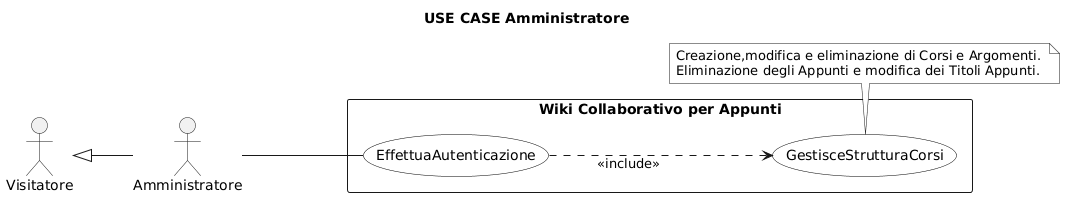
\includegraphics[width=1\textwidth]{UseCase/admin.png} % [10, 11]
    \caption{UC3 - Diagramma dei casi d'uso per l'attore Amministratore}
    \label{fig:uc_amministratore} % [12, 13]
\end{figure}

\begin{table}[H]
    \small
    \caption{Specifica del caso d'uso per RF2: EffettuaAutenticazione (Admin)}
    \label{tab:spec_uc2_admin}
    \begin{tabularx}{\textwidth}{@{}l X@{}}
        \toprule
        \textbf{ID} & 2 \\
        \midrule
        \textbf{Nome} & \textbf{EffettuaAutenticazione (Admin)} \\
        \midrule
        \textbf{Descrizione} & Consente all'Amministratore di accedere all'area gestionale del Wiki tramite credenziali riservate. \\
        \midrule
        \textbf{Attori} & Amministratore. \\
        \midrule
        \textbf{Precondizioni} & Il sistema è operativo e l'Amministratore possiede credenziali valide memorizzate tramite hashing. \\
        \midrule
        \textbf{Flusso Principale} & 
        1. L'Amministratore inserisce email e password nella pagina di login. \newline
        2. Il sistema invia i dati al backend tramite richiesta POST. \newline
        3. Il backend valida le credenziali confrontandole con i dati nel DB. \newline
        4. Il sistema avvia una sessione con privilegi elevati (Admin). \\
        \midrule
        \textbf{Postcondizioni} & L'Amministratore è autenticato e viene reindirizzato alla dashboard di gestione (11). \\
        \midrule
        \textbf{Flussi Alternativi} & \textbf{A1. Credenziali non valide:} Il sistema nega l'accesso e restituisce un errore JSON (status 401 Unauthorized). \\
        \bottomrule
    \end{tabularx}
\end{table}




\begin{table}[H]
    \small
    \caption{Specifica del caso d'uso per RF11: GestisceStrutturaCorsi}
    \label{tab:spec_uc11}
    \begin{tabularx}{\textwidth}{@{}l X@{}}
        \toprule
        \textbf{ID} & 11 \\
        \midrule
        \textbf{Nome} & \textbf{GestisceStrutturaCorsi} \\
        \midrule
        \textbf{Descrizione} & Permette all'Amministratore di creare, modificare o eliminare corsi e i relativi argomenti associati. \\
        \midrule
        \textbf{Attori} & Amministratore. \\
        \midrule
        \textbf{Precondizioni} & L'Amministratore ha effettuato con successo l'autenticazione (2). \\
        \midrule
        \textbf{Flusso Principale} & 
        1. L'Amministratore seleziona "Gestione Corsi" dalla dashboard. \newline
        2. Il sistema mostra l'elenco dei corsi esistenti recuperati dal DB. \newline
        3. L'Amministratore sceglie di inserire un nuovo corso o di modificarne uno esistente. \newline
        4. L'Amministratore inserisce, modifica e elimina corsi e argomenti. L'amministratore modifica i titoli degli appunti e elimina gli appunti. \newline
        5. Il sistema invia i dati al backend tramite REST API. \newline
        6. Il backend aggiorna le tabelle relazionali nel database. \\
        \midrule
        \textbf{Postcondizioni} & La nuova struttura dei corsi è salvata in modo persistente e visibile a tutti gli utenti (\textbf{RF3, RF4, RF5}). \\
        \bottomrule
    \end{tabularx}
\end{table}

\newpage
\section{Matrice di tracciabilità}
\begin{table}[htbp]
    \centering
    \caption{Matrice di tracciabilità}
    \begin{tabular}{lccc}
        \toprule
        Requisito Funzionale & UC1 (Visit.) & UC2 (Stud.) & UC3 (Admin) \\
        \midrule
        RF1 (Registrazione)  & X &   &   \\
        RF2 (Login/Logout)   &   & X & X \\
        RF3 (Lista corsi)    & X &   &   \\
        RF4 (Lista Argomenti)      & X &   &   \\
        RF5 (Visualizza appunto)& X &   &   \\
        RF6 (Crea appunto)   &   & X &   \\
        RF7 (Modifica appunto)       &   & X &   \\
        RF8 (Gestione Cronologia)     &   & X &   \\
        RF9 (Ricerca)        & X &   &   \\
        RF10 (Gestione Admin.)&   &   & X \\
        \bottomrule
    \end{tabular}
\end{table}
